%Autor: Jürg Rast
%Datum: 04.04.2012
%Lizenz: CC BY-SA
%Grundversion von https://github.com/jrast/ELT4-Notizen/blob/master/tikzPictures/RET/ReaktanzLTyp.tex

%Geändert von: Simon Walker
%Datum: 15.04.2020
%Lizenz: CC BY-NC-SA


\usepgflibrary{shapes.misc}
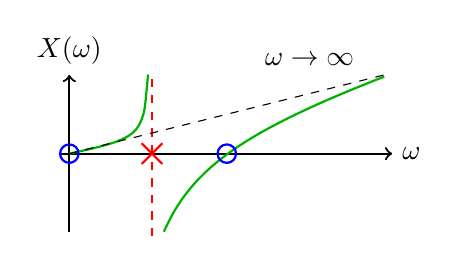
\begin{tikzpicture}[smooth, xscale=0.5, yscale=0.5]
% Achsen
\draw[->, thick] (-0.2,0) -- +(8.4,0) node[right] {$\omega$}; % Horizontal
\draw[->, thick] (0,-2) -- +(0,4) node[above] {$X(\omega)$}; % Vertikal

% Plots
\draw[color=green!70!black, thick] plot[domain=0:2] (\x,{\x/8+tan(\x*3/4 r)/8}); % Erster Tan
%\draw[color=green!70!black, thick] plot[domain=2.01:4.23] (\x,{tan(\x r)}); % zweiter Tan
\draw[color=green!70!black, thick] plot[domain=2.4:8] (\x,{ (\x/3.2) -3.8/(\x -1.01) }); % letzte kurve

% Poolstellen
\draw[dashed, thick, draw=red] (2.1,-2.1) -- +(0,4.2); % Poolstelle 1
\node[cross out, draw=red, thick] (wr1) at (2.1,0) {};


\draw[dashed] plot[domain=0:8] (\x, {\x/4});
\node (wL) at (6.1,2.4) {$\omega \rightarrow \infty$};

% Nullstellen
\node[rounded rectangle, draw=blue, thick] at(0,0) {};
\node[rounded rectangle, draw=blue, thick] at(4,0) {};
\end{tikzpicture}